%! Suppress = Unicode
\documentclass[a4paper,UKenglish,cleveref, autoref]{templates/lipics-v2019}
\usepackage{csquotes}
\usepackage{url}
\usepackage{pgfplots}
\usepackage{float}
%This is a template for producing LIPIcs articles.
%See lipics-manual.pdf for further information.
%for A4 paper format use option "a4paper", for US-letter use option "letterpaper"
%for british hyphenation rules use option "UKenglish", for american hyphenation rules use option "USenglish"
%for section-numbered lemmas etc., use "numberwithinsect"
%for enabling cleveref support, use "cleveref"
%for enabling cleveref support, use "autoref"

\newcommand{\sls}{Safer Language Subset}
\newcommand{\slss}{Safer Language Subsets}

\newcommand{\sqs}{Software-Qualitätsstandard}
\newcommand{\sqss}{Software-Qualitätsstandards}

\newcommand{\misra}{MISRA-C}

\graphicspath{{./graphics/}}%helpful if your graphic files are in another directory

\bibliographystyle{plainurl}% the mandatory bibstyle

\title{M10: \sqss}

\titlerunning{M10: \sqss}%optional, please use if title is longer than one line

\author{Alexander Linder}{Karlsruhe Institute of Technology, Germany \and \url{https://kit.edu} }{alexander.linder@student.kit.edu}{}{}
%mandatory, please use full name; first two parameters are mandatory, other parameters can be empty.

\authorrunning{A. Linder}
%mandatory. First: Use abbreviated first/middle names. Second (only in severe cases): Use first author plus 'et al.'

\Copyright{Alexander Linder}
%%mandatory, please use full first names. LIPIcs license is "CC-BY";  http://creativecommons.org/licenses/by/3.0/

\ccsdesc[100]{General and reference}
%mandatory: Please choose ACM 2012 classifications from https://dl.acm.org/ccs/ccs_flat.cfm

\keywords{\misra, \sqss}
%mandatory; please add comma-separated list of keywords

\category{}
%optional, e.g. invited paper

\relatedversion{}
%optional, e.g. full version hosted on arXiv, HAL, or other respository/website

\supplement{}
%optional, e.g. related research data, source code, ... hosted on a repository like zenodo, figshare, GitHub, ...

\funding{}
%optional, to capture a funding statement, which applies to all authors. Please enter author specific funding statements as fifth argument of the \author macro.

\acknowledgements{}
%optional

\nolinenumbers %uncomment to disable line numbering

\hideLIPIcs  %uncomment to remove references to LIPIcs series (logo, DOI, ...), e.g. when preparing a pre-final version to be uploaded to arXiv or another public repository

%Editor-only macros:: begin (do not touch as author)%%%%%%%%%%%%%%%%%%%%%%%%%%%%%%%%%%
\EventEditors{}
\EventNoEds{0}
\EventLongTitle{Proseminar Werkzeuge und Methoden der Software-Analyse}
\EventShortTitle{Proseminar}
\EventAcronym{Proseminar}
\EventYear{2019}
\EventDate{WS19/20}
\EventLocation{Karlsruhe, Deutschland}
\EventLogo{}
\SeriesVolume{}
\ArticleNo{M10}
%%%%%%%%%%%%%%%%%%%%%%%%%%%%%%%%%%%%%%%%%%%%%%%%%%%%%%

\begin{document}

    \maketitle

    %TODO mandatory: add short abstract of the document
    \begin{abstract}
        Diese Arbeit gibt einen Überblick über \sqss\ im Allgemeinen sowie unter besonderer Betrachtung eines weitverbreiteten Beispiels, \misra\ 2004.\\
        Es wird die hinter \sqss\ stehende Motivation dargebracht, sowie betrachtet wie sich Regeln innerhalb eines Standards sinnvoll klassifizieren lassen.
        Dies führt zum Begriff des \slss\ nach Hatton~\cite{hatton2004safer}, welches formale Forderungen an einen guten Regelsatz aufstellt.
        Weiterhin wird überprüft, inwiefern \misra\ diese Definition erfüllt.\\
        Final sollen Gütekriterien für \sqss\ aufgestellt werden und die Güte des \misra\ Standards unter eben diesen Kriterien bewertet werden.
    \end{abstract}

    \section{Einleitung}
    \label{sec:einleitung}

    \section{\misra}
    \label{sec:misra-c}
    \misra\ ist ein weitverbreiteter \sqs, der von der \textbf{M}otor \textbf{I}ndustry \textbf{S}oftware \textbf{R}eliability \textbf{A}ssociation (MISRA) entwickelt wurde.
    Die erste Version von \misra\ wurde 1998 veröffentlicht, mit insgesamt zwei großen Revisionen einmal 2004 sowie 2012,
    wobei sich diese Arbeit auf die Standards von 1998 (künftig M1998) und 2004 (künftig M2004) beschränkt, da einerseits der Standard von 2004 nach wie vor
    weite Verbreitung findet und sich andererseits die Forschung auf diese beiden Versionen konzentriert.\\
    Bei \misra\ handelt es sich um den de facto Standard zur Programmierung eingebetteter Systeme in der Mehrheit der sicherheitsrelevanten Industrien in der Programmiersprache C\@.\cite{misra-website}
    Sowohl M1998 als auch M2004 nehmen Bezug nehmen Bezug auf C89/90 und nicht auf den neueren C-Standard C99 (ISO/IEC9899:1999), was dazu führt, dass neuere Sprachkonstrukte in
    \misra-konformem Code nicht erlaubt sind, auch wenn die verwendeten Compiler sie unterstützen.

    \subsection{Evolution des Standards}
    \label{subsec:evolution-des-standards}

    \begin{figure}[H]
        \centering
        \captionsetup{justification=centering,margin=2cm}
        \begin{tikzpicture}[scale=0.7]
    \pie[sum=auto]{93/ , 34/ }
    \pie[pos={8,0},sum=auto, text=legend]{122/verpflichtend, 20/empfohlen}
\end{tikzpicture}
        \caption{Regelanzahl 1998 vs 2004}
    \end{figure}

    \subsection{Beispielregel}
    \label{subsec:beispielregel}

    \noindent
    \begin{minipage}{\linewidth}
        \begin{example}
            \textbf{Rule 2.1 (required): Assembly language shall be encapsulated and isolated\cite{MISRA2004}}\\
            Where assembly language instructions are required it is recommended that they be encapsulated
            and isolated in either (a) assembler functions, (b) C functions or (c) macros.\\
            For reasons of efficiency it is sometimes necessary to embed simple assembly language instructions
            in-line, for example to enable and disable interrupts.
            If it is necessary to do this for any reason, then it is recommended that it be achieved by using macros.\\
            Note that the use of in-line assembly language is an extension to standard C, and therefore also
            requires a deviation against Rule 1.1.
            \begin{lstlisting}[language=C]
                #define NOP asm(" NOP")
            \end{lstlisting}
        \end{example}
    \end{minipage}

    \section{Regelklassifizierung}
    \label{sec:regelklassifizierung}
    In diesem Abschnitt wollen wir untersuchen, wie wir Regeln eines Regelsatzes sinnvoll klassifizieren können.
    Hierfür gibt es viele verschiedene Möglichkeiten.
    Im vorigen Abschnitt haben wir bereits gesehen, wie der Regelsatz von \misra\ organisiert wird.
    Hierbei handelte es sich schlicht um eine thematische Organisation der Regeln in Gruppen.
    Wir wollen nun eine alternative Klassifikationsart betrachten, die nicht auf dem Inhalt der Regeln, sondern auf ihrer
    Art sowie dem Grad an Evidenz, der ihre Existenz begründet, basiert.
    Regeln werden in diesem System in drei Typen unterschieden, einserseits Typ-A (\enquote{Style-basierte}) Regeln,
    sowie Typ-B (\enquote{funktionale}) Regeln, welche sich weiter in Typ-B.1 (\enquote{Subjektive}) sowie
    Typ B.2 (\enquote{Evidente}) unterscheiden lassen.\cite{hatton2004safer}

    \subsection{Typ-A Regeln}
    \label{subsec:typ-a-regeln}
    \begin{definition}
        Eine Typ A Regel sei eine Regel, welche alleinig den Stil des Codes beeinflusst.
    \end{definition}

    \noindent
    \begin{minipage}{\linewidth}
        \begin{example}
            \lstinputlisting[title=\ ]{graphics/typa.c}
        \end{example}
    \end{minipage}

    \subsection{Typ-B.1 Regeln}
    \label{subsec:typ-b-1-regeln}
    \begin{definition}
        Eine Typ B.1 Regel sei eine Regel, welche potentiell unsichere Sprachfeatures ausschließt,
        jedoch keine empirischen Daten besitzt, die diesen Ausschluss begründen.
    \end{definition}

    \noindent
    \begin{minipage}{\linewidth}
        \begin{example}
            \lstinputlisting[title=\ ]{graphics/typb1.c}
        \end{example}
    \end{minipage}
    
    \subsection{Typ-B.2 Regeln}
    \label{subsec:typ-b-2-regeln}
    \begin{definition}
        Eine Typ B.2 Regel sei eine Regel, welche potentiell unsichere Sprachfeatures ausschließt und empirische
        Daten besitzt, die diesen Ausschluss begründen.
    \end{definition}

    \noindent
    \begin{minipage}{\linewidth}
        \begin{example}
            \lstinputlisting[title=\ ]{graphics/typb2.c}
        \end{example}
    \end{minipage}
    
    \section{Safer Language Subsets}
    \label{sec:safer-language-subsets}
    \begin{definition}
        Ein Regelsatz $R$ sei ein \sls $\iff$
        \begin{itemize}
            \item $R$ enthält nur Typ B.2 Regeln als verpflichtende Regeln
            \item $R$ enthält nur Typ B.1 Regeln als empfohlene Regeln
            \item $R$ enthält keinerlei Typ A Regeln
        \end{itemize}
        
    \end{definition}
    
    \section{Bewertung}
    \label{sec:bewertung}

    \subsection{Signal-Rausch-Rate}
    \label{subsec:signal-rausch-rate}

    \begin{definition}
        Die Prävalenz (\enquote{base rate}) mit der bekannte Fehlerquellen von Programmiersprachen auftreten bezeichnen wir mit $B$.
    \end{definition}

    \begin{definition}
        Die Erkennungsrate (\enquote{detection rate}) eines Standards ist die gesamte Anzahl an Abweichungen pro 1000 Zeilen
        ausführbaren Codes gemeint ist.
        Wir bezeichnen sie mit $D$.
    \end{definition}
    
    \begin{definition}
        Wir definieren die Signal-Rausch-Rate $S$, also die Rate in der bekannte Defekte gefunden werden, als:
        \begin{equation*}
            S=B/D
        \end{equation*}
    \end{definition}

    \begin{figure}[H]
        \centering
        \captionsetup{justification=centering,margin=2cm}
        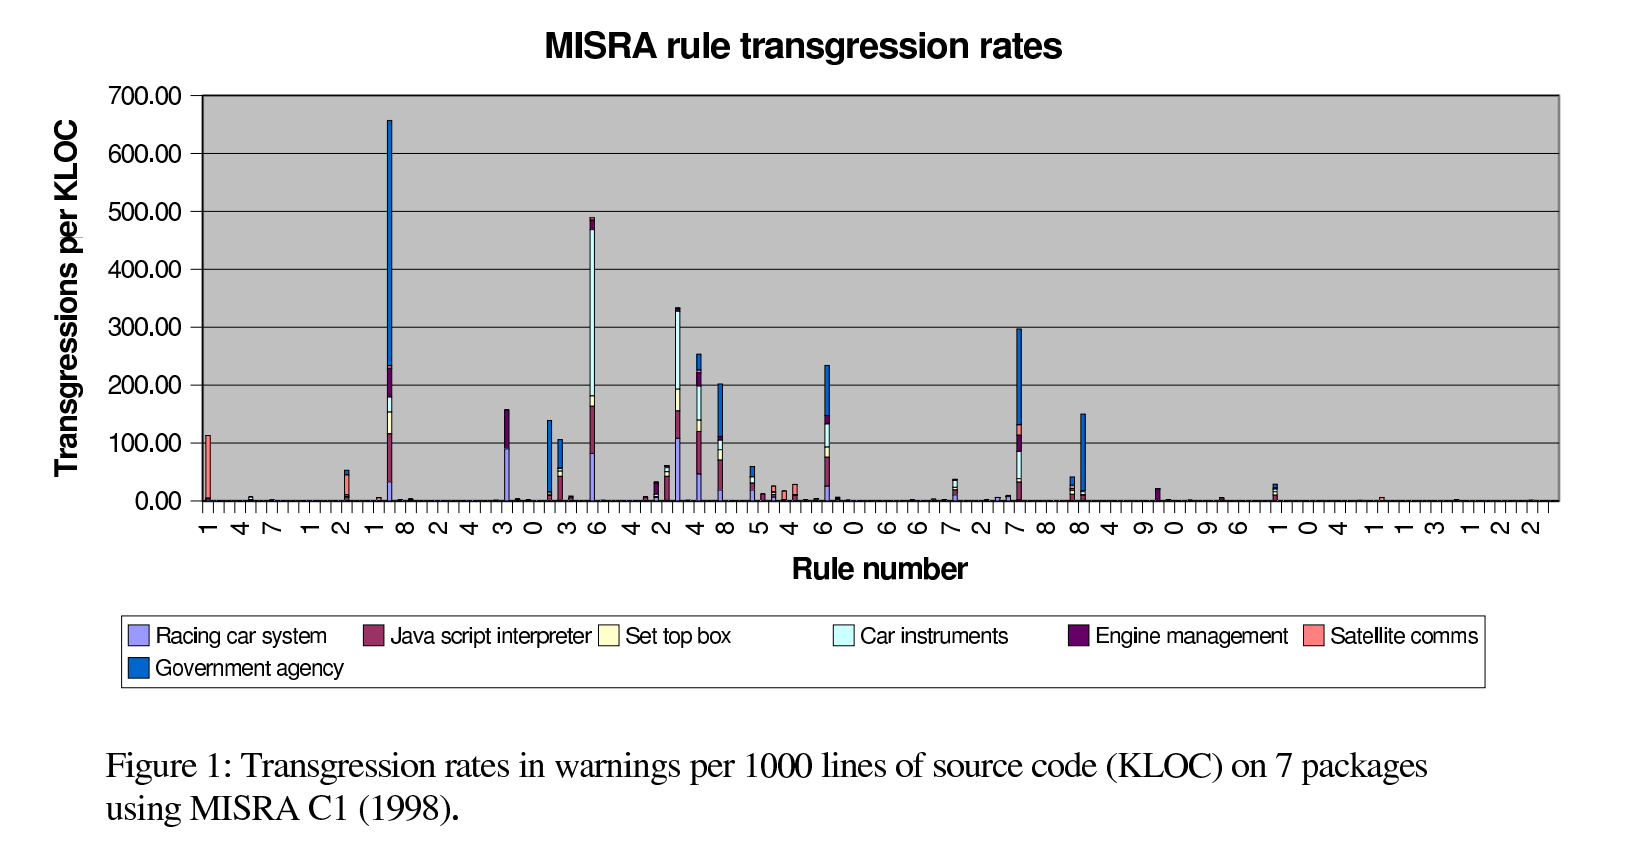
\includegraphics[width=\textwidth]{graphics/1998-transgression-rates.png}
        \caption{Verstöße in Warnungen je 1000 Codezeilen auf 7 Pakete verteilt, M1998\cite{hatton2007language}}
    \end{figure}

    \begin{figure}[H]
        \centering
        \captionsetup{justification=centering,margin=2cm}
        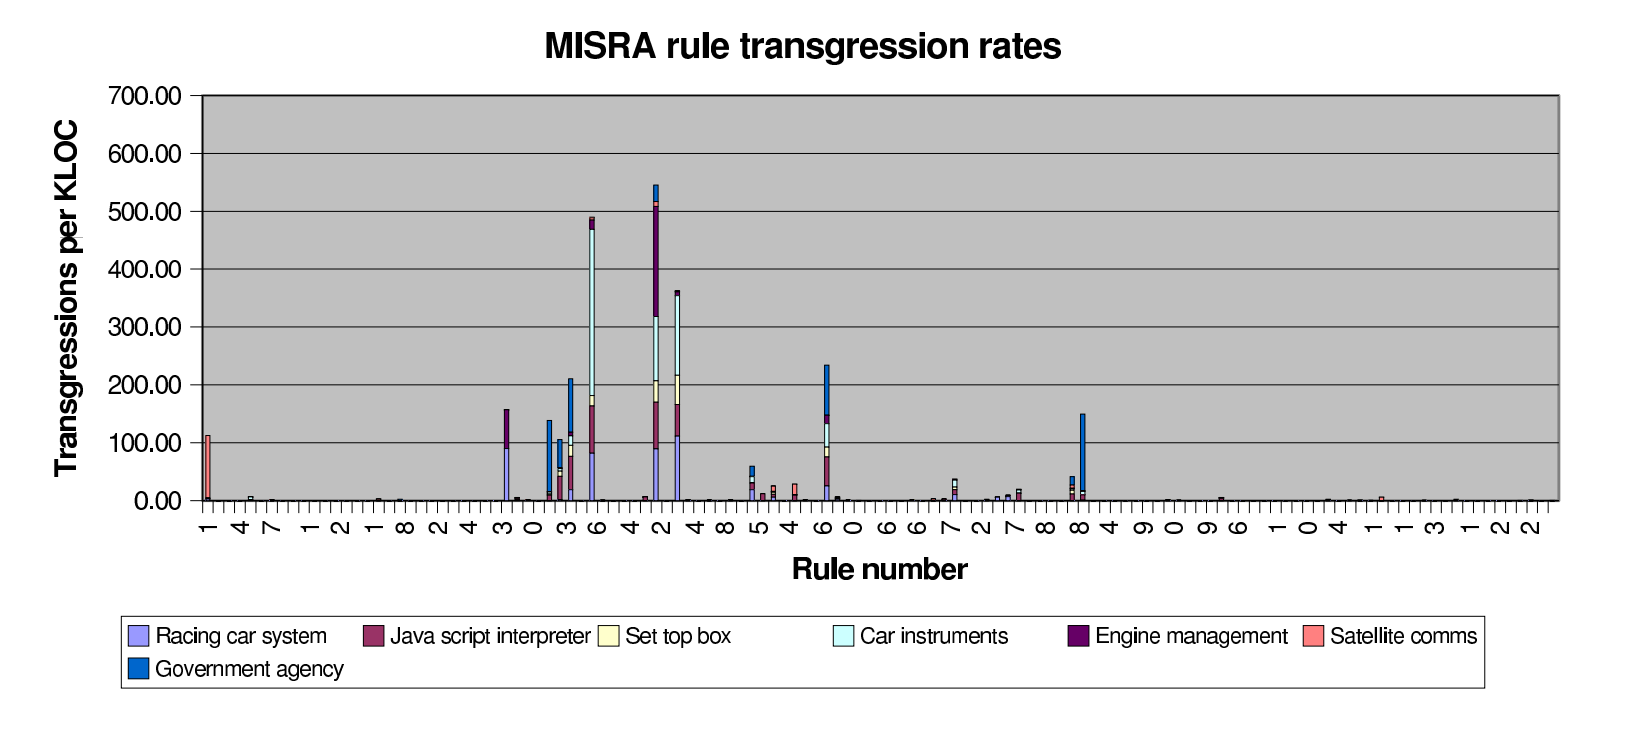
\includegraphics[width=\textwidth]{graphics/2004-transgression-rates.png}
        \caption{Verstöße in Warnungen je 1000 Codezeilen auf 7 Pakete verteilt, M2004\cite{hatton2007language}}
    \end{figure}

    \section{Konklusion}
    \label{sec:konklusion}

    %%
    %% Bibliography
    %%

    %% Please use bibtex,

    \bibliography{prosem}

\end{document}
